\section{Capacitores em C.C. e C.A.}

\frame{
	\frametitle{O capacitor}
	\begin{block}{Introdução}
		O capacitor é um componente que tem a finalidade de armazenar cargas elétricas. É constituído por duas placas condutoras separadas por um material isolante (dielétrico).
	\end{block}
	\centerline{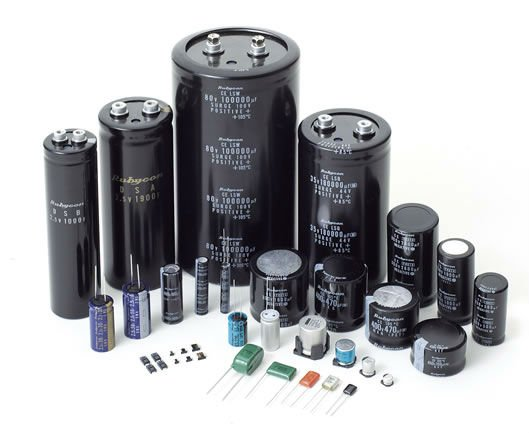
\includegraphics[width=0.5\linewidth]{Figuras/Ch12/capacitores.jpg}}
}

\frame{
	\frametitle{Capacitância}
	\begin{block}{Aspectos construtivos}
		\begin{itemize}
			\item Capacitância ($C$) é a característica de armazenamento
			\item A capacitância depende da geometria do capacitor (de placas paralelas, cilíndrico, esférico). Para um determinado material, a capacitância dependerá somente de suas dimensões: quanto maiores forem, maior será a capacitância.
			\item A capacitância se verifica sempre que dois condutores estiverem separados por um material isolante. Assim, a capacitância depende do dielétrico que se introduza entre as duas superfícies do capacitor. Quanto maior for a constante dielétrica do material não condutor introduzido, maior será a capacitância.
		\end{itemize}
	\end{block}
}

\frame{
	\frametitle{Capacitância}
	\begin{block}{Relação matemática}
		$$C = \dfrac{Q}{U} \qquad [\si{\farad}]$$
	\end{block}

	\vspace{1.5cm}

	\setmyunit{2cm}
	
	\centering
	\begin{circuitikz}
		\draw (0,0) to[short,o-] ++(0.5,0)
		to[C,l=$ C $,v=$ {} $,*-*] ++(0,-1)
		to[short,-o] ++(-0.5,0) (0.5,0) -- ++(1,0)
		to[R,l=$ R $,*-*] ++(0,-1) -- ++(-1,0);
		\draw[decorate,decoration={brace,amplitude=10pt,mirror},xshift=-5pt] (0,0) -- node[left=8pt] {$ U $} (0,-1);
	\end{circuitikz}
%	\centerline{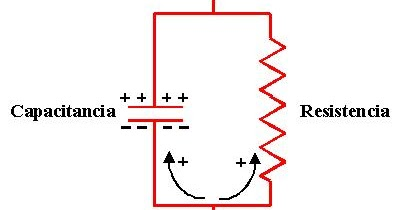
\includegraphics[width=0.6\linewidth]{Figuras/Ch12/capacitancia.jpg}}
}

\frame{
	\frametitle{Transitório: fase de carga}
	\setmyunit{2cm}
	\centering
	\begin{circuitikz}[scale=0.9]
		\draw (2,0) to[battery,v=$  $,l_=$ \epsilon $] ++(0,-2) -- ++(1.5,0);
		\begin{scope}[european voltages]
			\draw (2,0) to[nos,l=$ S $] ++(1.5,0)
			to[R,l=$ R $,v=$ V_R $] ++(0,-1)
			to[C,l=$ C $,v=$ V_C $] ++(0,-1);
		\end{scope}
	\end{circuitikz}
	
%	\centerline{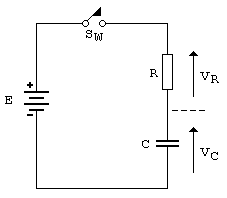
\includegraphics[width=0.4\linewidth]{Figuras/Ch12/capacitorcc.jpg}}
	\begin{block}{Capacitor em regime C.C.}
		\begin{itemize}
			\item No instante em que a chave é fechada, a bateria começa a remover elétrons da placa superior e depositá-los na placa inferior.
			\item Eventualmente, quando a tensão entre os terminais do capacitor se iguala à tensão da bateria, cessa o movimento de elétrons.
		\end{itemize}
	\end{block}
}

\frame{
	\frametitle{Transitório: fase de carga}
	\setmyunit{2cm}
	\centering
	\begin{circuitikz}[scale=0.9]
		\draw (2,0) to[battery,v=$  $,l_=$ \epsilon $] ++(0,-2) -- ++(1.5,0);
		\begin{scope}[european voltages]
			\draw (2,0) to[nos,l=$ S $] ++(1.5,0)
			to[R,l=$ R $,v=$ v_R $] ++(0,-1)
			to[C,l=$ C $,v=$ v_C $] ++(0,-1);
		\end{scope}
	\end{circuitikz}
%	\centerline{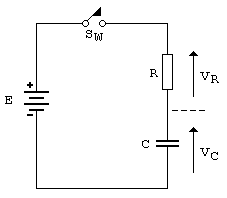
\includegraphics[width=0.4\linewidth]{Figuras/Ch12/capacitorcc.jpg}}
	\begin{block}{$t=0$}
		\begin{itemize}
			\item A corrente continuará fluindo pelo circuito até que o capacitor fique completamente carregado.
			\item A corrente será máxima, dada por $i = \dfrac{\epsilon}{R}$
		\end{itemize}
	\end{block}
}

\frame{
	\frametitle{Transitório: fase de carga}
	\setmyunit{2cm}
	\centering
	\begin{circuitikz}[scale=0.9]
		\draw (2,0) to[battery,v=$  $,l_=$ \epsilon $] ++(0,-2) -- ++(1.5,0);
		\begin{scope}[european voltages]
			\draw (2,0) to[nos,l=$ S $] ++(1.5,0)
			to[R,l=$ R $,v=$ v_R $] ++(0,-1)
			to[C,l=$ C $,v=$ v_C $] ++(0,-1);
		\end{scope}
	\end{circuitikz}

%	\centerline{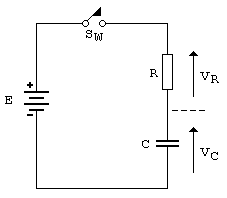
\includegraphics[width=0.4\linewidth]{Figuras/Ch12/capacitorcc.jpg}}
	\begin{block}{$t=0^+$}
		\begin{itemize}
			\item A tensão no resistor será igual a tensão da bateria, pois o capacitor ainda está descarregado.
			\item A corrente vai diminuindo dada por $i = \dfrac{\epsilon-v_C}{R}$
		\end{itemize}
	\end{block}
}

\frame{
	\frametitle{Transitório: fase de carga}
	\setmyunit{2cm}
	\centering
	\begin{circuitikz}[scale=0.9]
		\draw (2,0) to[battery,v=$  $,l_=$ \epsilon $] ++(0,-2) -- ++(1.5,0);
		\begin{scope}[european voltages]
			\draw (2,0) to[nos,l=$ S $] ++(1.5,0)
			to[R,l=$ R $,v=$ v_R $] ++(0,-1)
			to[C,l=$ C $,v=$ v_C $] ++(0,-1);
		\end{scope}
	\end{circuitikz}

%	\centerline{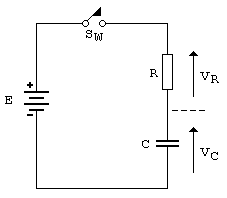
\includegraphics[width=0.4\linewidth]{Figuras/Ch12/capacitorcc.jpg}}
	\begin{block}{$t=\infty$}
		\begin{itemize}
			\item Em um tempo suficientemente grande temos que $V_C = \epsilon$
			\item A corrente é nula, i.e., $i=\SI{0}{\ampere}$
		\end{itemize}
	\end{block}
}

\frame{
	\frametitle{Constante de tempo}
	\centerline{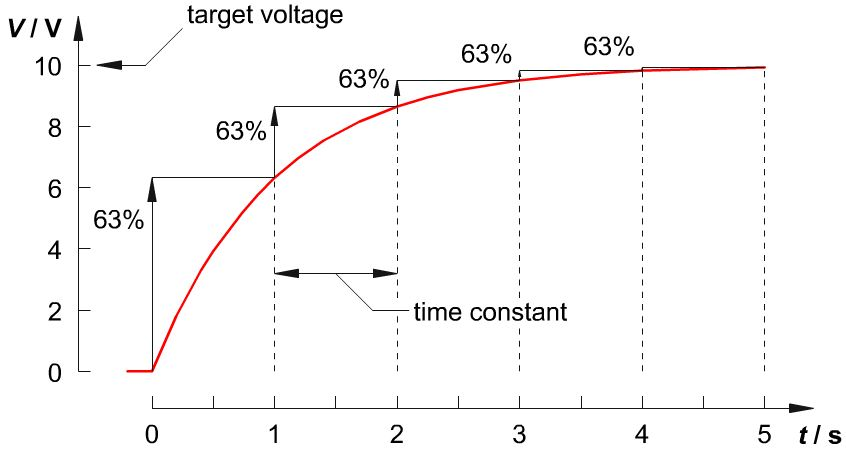
\includegraphics[width=0.7\linewidth]{Figuras/Ch12/capacitor-charging-graph.jpg}}
	\begin{block}{Constante de tempo}
		O fator $\tau$, chamado de constante de tempo do circuito, tem a unidade de tempo e pode ser calculada como:
		$$\tau = RC$$
	\end{block}
}

\frame{
	\frametitle{Transitório: fase de carga}
	\centerline{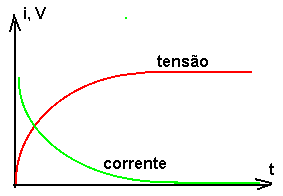
\includegraphics[width=0.4\linewidth]{Figuras/Ch12/tensaocorrentecarga.png}}
	\begin{block}{Curva de carga - corrente}
		\[ i_C(t) = \dfrac{\epsilon}{R} \Big( \text{e}^{-t/\tau} \Big) \]
		\begin{itemize}
			\item a corrente de um circuito C.C. capacitivo é essencialmente zero ampère após cinco constantes de tempo da fase de carga terem passado.
		\end{itemize}
	\end{block}
}

\frame{
	\frametitle{Transitório: fase de carga}
	\centerline{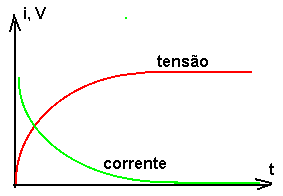
\includegraphics[width=0.4\linewidth]{Figuras/Ch12/tensaocorrentecarga.png}}
	\begin{block}{Curva de carga - tensão}
		\[ v_C = \epsilon - Ri(t) \implies v_C = \epsilon - \cancel{R} \cdot \dfrac{\epsilon}{\cancel{R}} \Big( \text{e}^{-t/\tau} \Big)  \implies v_C(t) = \epsilon\Big( 1-\text{e}^{-t/\tau}\Big) \]
		\begin{itemize}
			\item a tensão através de um capacitor em um circuito C.C. é essencialmente igual à tensão aplicada após cinco constantes de tempo da fase de carga.
		\end{itemize}
	\end{block}
}

\frame{
	\frametitle{Transitório: fase de carga}
	\begin{block}{Conclusões}
		\begin{itemize}
			\item Um capacitor pode ser substituído por um circuito aberto equivalente assim que a fase de carga em um circuito C.C. tiver passado.
			\item Um capacitor tem as características de um curto-circuito equivalente no instante em que a chave é fechada em um circuito RC em série.
		\end{itemize}
	\end{block}
}

\frame{
	\frametitle{Transitório: fase de descarga}
	\centerline{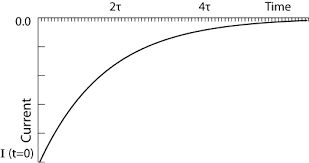
\includegraphics[width=0.7\linewidth]{Figuras/Ch12/correntedescarga.png}}
	\begin{block}{Curva de descarga - corrente}
		\[ i_C(t) = \dfrac{\epsilon}{R} \Big( \text{e}^{-t/\tau} \Big) \]
	\end{block}
}

\frame{
	\frametitle{Transitório: fase de descarga}
	\centerline{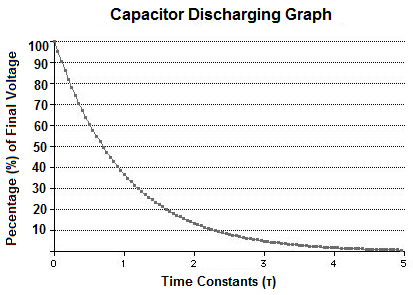
\includegraphics[width=0.6\linewidth]{Figuras/Ch12/tensaodescarga.png}}
	\begin{block}{Curva de descarga - tensão}
		\[ v_C(t) = \epsilon \Big( \text{e}^{-t/\tau} \Big) \]
	\end{block}
}

\frame{
	\frametitle{Capacitores em regime C.A.}
	\begin{block}{Reatância capacitiva}
		A reatância capacitiva é uma oposição à corrente que resulta em uma troca contínua de energia entre a fonte e o campo elétrico do capacitor. Sua relação é dada por: \\
		$$X_C = \dfrac{1}{2\pi fC} \qquad[\si{\ohm}]$$ \\
		\begin{itemize}
			\item À medida que a frequência aumenta, a reatância capacitiva decresce até atingir um valor praticamente nulo.
		\end{itemize}
	\end{block}
}

\frame{
	\frametitle{Capacitores em regime C.A.}
	\begin{block}{Tensão e corrente do capacitor}
		Lembrando que quando o capacitor está descarregado ($v_C = \SI{0}{\volt}$), a corrente
		é máxima; e quando carregado ($v_C = V_{\text{máx}}$), a corrente é nula.
	\end{block}
}

\frame{
	\frametitle{Capacitores em regime C.A.}
	\begin{block}{Tensão e corrente do capacitor}
		$$i(t) = i_{\text{máx}} \sen \left( \omega t + \dfrac{\pi}{2}\right)  \quad \text{onde } i_{\text{máx}} = \dfrac{V_{\text{máx}}}{X_C}$$
	\end{block}
	\centerline{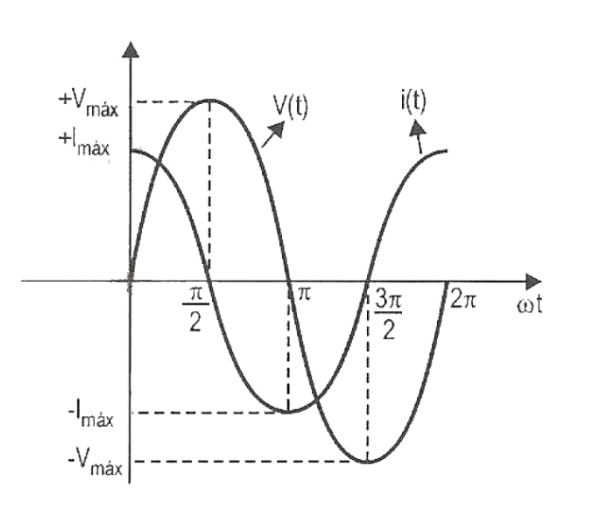
\includegraphics[width=0.45\linewidth]{Figuras/Ch12/tensaocorrente.PNG}}
	\vspace{-0.5cm}
	\begin{block}{Conclusão}
		Dizemos que a \textbf{corrente está adiantada $\ang{90}$ em relação a tensão.}
	\end{block}
}

\frame{
	\frametitle{Circuitos RC série}
	\setmyunit{2cm}
	\centering
	\begin{circuitikz}
		\draw (1,0) to[sV,l_=$ V $] ++(0,-1.5) -- ++(1.5,0)
		(1,0) to[R,l=$ R $] ++(1.5,0)
		to[C,l=$ X_C $] ++(0,-1.5);
	\end{circuitikz}

%	\centerline{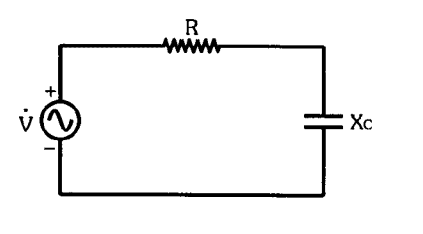
\includegraphics[width=0.6\linewidth]{Figuras/Ch12/rcserie.PNG}}
	\begin{block}{Impedância}
		Todo circuito em regime A.C. oferece uma oposição à passagem de corrente elétrica denominada impedância ($Z$) medida em ohms ($\si{\ohm}$). No circuito RC série a impedância é a soma vetorial de $R$ e $X_c$
	\end{block}
}

\frame{
	\frametitle{Circuitos RC série}
	\setmyunit{2cm}
	\centering
	\begin{circuitikz}[scale=0.7]
		\draw (1,0) to[sV,l_=$ V $] ++(0,-1.5) -- ++(1.5,0)
		(1,0) to[R,l=$ R $] ++(1.5,0)
		to[C,l=$ X_C $] ++(0,-1.5);
	\end{circuitikz}

%	\centerline{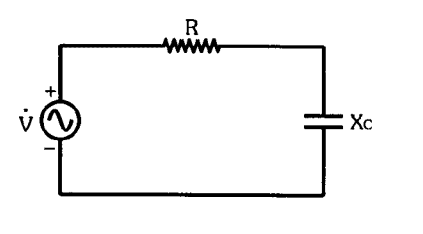
\includegraphics[width=0.4\linewidth]{Figuras/Ch12/rcserie.PNG}}
	\begin{block}{Formulações}
		\begin{gather*}
			Z = \sqrt{R^2 + X_C^2}\\
			\phi = - \arctg \left( \dfrac{X_C}{R}\right) \\
			i_{\text{ef}} = \dfrac{V_{\text{ef}}}{Z}\\
			V_{\text{Ref}} = R \cdot i_{\text{ef}}\\
			V_{\text{Cef}} = X_c \cdot i_{\text{ef}}
		\end{gather*}
	\end{block}
}

\section*{Exercícios}

\frame{
	\frametitle{Exercícios}
	\begin{block}{}
		01. Esboce o diagrama vetorial de um circuito RC série considerando uma fonte de tensão alternada de \SI{100}{\voltef} com frequência \SI{60}{\hertz}, $C = \SI{0.1}{\micro\farad}$ e $R = \SI{10}{\kilo\ohm}$.

		\vspace{1cm}

		02. A expressão para a tensão em um capacitor de $\SI{1}{\micro\farad}$ é $v(t) = 30 \sen(400t)$. Qual é a expressão senoidal para a corrente?

		\vspace{1cm}

		03. Um resistor de \SI{6.2}{\mega\ohm} e um capacitor de \SI{2.4}{\micro\farad} são conectados em série a uma bateria de \SI{12}{\volt}, de resistência interna desprezível. (a) Qual é a constante de tempo capacitiva deste circuito? (b) Em que instante após a bateria ser conectada, o valor da tensão no capacitor é igual \SI{5.6}{\volt}?

	\end{block}
}

\section*{Referências}

\frame{
	\frametitle{Referências e Exercícios Complementares}
	\begin{itemize}
		\item ALEXANDRE, Charles K.; SADIKU, Matthew N. O. Fundamentos de Circuitos Elétricos. 5. ed. Porto Alegre: AMGH, 2013.
	\end{itemize}
	%\centering{\alert{Página 36 - \textbf{1.6.1 até 1.6.5, 1.6.17 até 1.6.19}}} \\
	\centering{\alert{Lista de exercícios 12}}
}